\documentclass{article}%
\usepackage[T1]{fontenc}%
\usepackage[utf8]{inputenc}%
\usepackage{lmodern}%
\usepackage{textcomp}%
\usepackage{lastpage}%
\usepackage{authblk}%
\usepackage{graphicx}%
%
\title{Cyclin D1 cooperates with p21 to regulate TGFb{-}mediated breast cancer cell migration and tumor local invasion}%
\author{Natasha Mcbride}%
\affil{Zhang Zhongjing College of Chinese Medicine, Nanyang Institute of Technology, China}%
\date{01{-}01{-}2007}%
%
\begin{document}%
\normalsize%
\maketitle%
\section{Abstract}%
\label{sec:Abstract}%
Abstract\newline%
Genetic toxicity is a significant concern for patients diagnosed with peripheral neuropathy, and as a primary treatment modality that has proven safe and efficacious in laboratory animals. Therefore, a team of researchers led by Mark Greinelder from Scripps Research Laboratories, Inc. involved in the design of recombinant microspheres derived from a pluripotent stem cell derived from growth factors seen on the cell surface of cells underwent a randomized controlled trial involving 13 adult patients suffering from peripheral neuropathy. The study represents the first research to directly assess the effects of trans10{-}cis12 conjugated linoleic acid (10{-}cis12) in phagocytosis of mature macrophages via a peroxisome proliferator{-}activated receptor gamma{-}dependent pathway on peroxiocytosis of mature macrophages. The authors completed a successful Phase I/II clinical trial consisting of 0.3 arm partial treatment, 0.6 arm curative chemotherapy treatment, and 24{-}day maintenance of a quinine inhibitor, demonstrating that trans10{-}cis12 conjugated linoleic acid (10{-}cis12) works as the pathway by which MD/PD kinase (MPDK1) is subcutaneously initiated to stimulate growth of macrophages, leading to development of cancerous tumors.

%
\subsection{Image Analysis}%
\label{subsec:ImageAnalysis}%


\begin{figure}[h!]%
\centering%
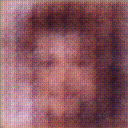
\includegraphics[width=150px]{500_fake_images/samples_5_432.png}%
\caption{A Black And White Photo Of A Black And White Cat}%
\end{figure}

%
\end{document}